\chapter{Data Layout}
\label{chap:Data Layout}
One of the most prevalent ways of achieving good performance for OLAP workloads, is to consider how the data is laid out in all levels of the memory hierarchy. Most of the discussion relates to column stores against row stores, but we see alternate ways of storing the data. In addition to the overall storage format, one should also consider if and how to partition the data, and how to sort it.
\newpage

%\ffigure{img/row-store.png}{Row-oriented layout for example tuples. Courtesy of \cite{Bjorklund2011-wh}.}{fig:row-store}
%\ffigure{img/column-store.png}{Column-oriented layout for example tuples. Courtesy of \cite{Bjorklund2011-wh}.}{fig:column-store}
\begin{figure}
  \centering
  \begin{subfigure}{\textwidth}
    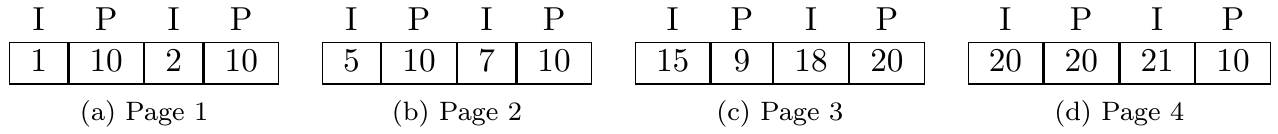
\includegraphics[width=\textwidth]{img/row-store.png}
    \caption{Row store layout.}
    \label{fig:row-column-store-1} 
  \end{subfigure}
  \begin{subfigure}{\textwidth}
    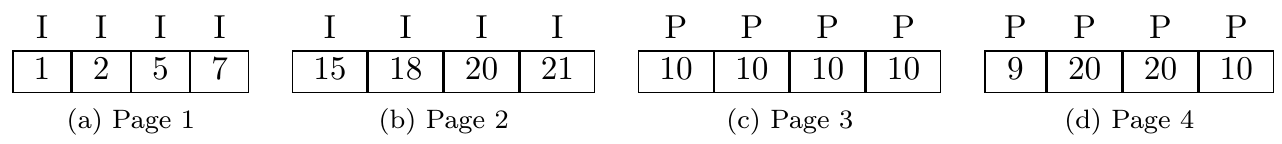
\includegraphics[width=\textwidth]{img/column-store.png}
    \caption{Column store layout.}
    \label{fig:row-column-store-2} 
  \end{subfigure}
  \caption{Row and column oriented layouts for a table with two columns, I and P. In the row-oriented layout (a), records (I and P tuples) are stored next to each other within the pages. In the column-oriented layout (b), values from the I column and P column are stored separately on different pages. Courtesy of \cite{Bjorklund2011-wh}.}
  \label{fig:row-column-store} 
\end{figure}
\section{Column Storage}
\label{sec:Column Storage}


The most common storage format for OLTP systems is row storage, as we briefly mentioned in Section \ref{sec:Definitions}. Row storage enables easy fetching of related data and is suited for updates, inserts, and deletes. However for OLAP workloads, columnar storage has turned out advantageous, mainly because of two reasons: First, aggregations are easier, since calculations are performed on data consecutive in memory. Second, column storage does not fetch more data than is needed for the query.

Our research have identified several systems using columnar storage. These include \monetdb~\cite{Boncz2002-yj, Boncz2005-wj}, \cstore~\cite{Stonebraker2005-qz}, \saph~\cite{Farber2012-vh}, and \mssql~\cite{noauthor_undated-vq, Larson2013-mc}, as well as the \bd~product Tableau \cite{Kamkolkar2015-iq}.

In a column store, each column in a table is stored separately in a continuous segment (unless data is horizontally partitioned, see Section \ref{sec:Horizontal Partitioning}), as opposed to row stores where attributes from a single row are stored together \cite{Bjorklund2011-wh}. Figure \ref{fig:row-column-store} depicts both row and column oriented layouts for a table with two columns (I and P). The row storage alternates between I and P to store records next to each other on the pages while the column storage keeps I and P values separate. 

The advantages of using column storage are many, where the primary advantage is that no more data is accessed than strictly necessary. In addition to this, columns are inherently more compressible \cite{noauthor_undated-vq}. Compression leads to higher performance due to better cache and memory utilization, and this effect is one of the reasons why \mssql~use column storage. We elaborate on the effects of compression in Chapter \ref{chap:Data Compression}.

Column storage also comes with a more subtle advantage that is that columns have a \textit{low degree of freedom} \cite{Boncz2005-wj}. When operating on column values, only the local memory offset is required, not the global table layout. This removes some layers of indirection and query processing can be made more efficient. Boncz \ea~claim that this is the main reason why column storage is advantageous.


One of the major disadvantages with column store is that it is not as easily updateable \cite{Bjorklund2011-wh}, especially if the columns are compressed or sorted. This challenge is normally overcome using a separate structure for writes and updates called a \textit{delta store}. Using such structure, the main part of the database is stored column-wise in a static structure optimized for reads while the updates and inserts are accumulated in a smaller and more dynamic structure. We investigate delta stores further in Section \ref{sub:Delta Store}.

Another disadvantage with column storage is tuple materialization costs. Since the result of most DBMS queries should be returned as rows, columns must be stitched back together before returned to the client, an operation that can be expensive.


\subsection{Sorting}
\label{sub:Sorting}
We see that few systems sort the data values before storing them to columns. An exception to this is \cstore, and later \vertica~\cite{Lamb2012-kg, Stonebraker2005-qz}. In these systems, \textit{column projections} can be defined, which is a subset of the columns in a table. Each column projection is sorted based on one column in the subset, which means a column is either sorted by own values or simply sorted by values from another column in the projection. Projections are specified by the database administrator. A column can have multiple projections, hence multiple sort orders, which results in data duplication. The extra storage needed for multiple column sort orders is justified by the compression that column storage enables.


Sorting values in a column store comes with some advantages. First, single value lookups are easily performed by a binary search (however, this limitation can be overcome by keeping inverted indexes \cite{Lemke2010-is, Schwalb2014-hn}, which we study in Section \ref{sec:Inverted Indexes}) Second, and perhaps most important, is that sorted columns can be compressed aggressively by applying \rle. \rle~is the main reason \cstore~stores sorted data \cite{Stonebraker2005-qz}. We study this type of compression in Section \ref{sec:Run-Length Encoding}.

Column sorting also comes with a performance benefit. Holloway \ea~show how sorted columns perform better due to \rle~\cite{Holloway2008-rr}. \blink~has also reported a performance increase if the columns are sorted prior to testing \cite{Johnson2008-cp}, even if this system does not use \rle.

Except from \cstore~and \vertica, our research has shown little indication that sorting values in columns are common. For instance, \mssql~\cite{Larson2013-mc}, \blink~\cite{Raman2013-em} and \oracle~\cite{Lahiri2015-mz} accept values in the order they appear.

Although most systems do not sort values in the columns, that is values are insert in the same order as they arrive, many systems have a sorted dictionary when dictionary encoding is used. Systems here include \blink~\cite{Johnson2008-cp} and \saph~\cite{Farber2012-vh}. A sorted dictionary has many advantages, like easy lookup for single values, transformation of range predicates to \texttt{IN}-list predicates, and partition pruning. A sorted dictionary structure is better suited for a read-only environment, since updating a sorted dictionary requires some work. We look into dictionary encoding in Section \ref{sec:Dictionary Encoding}.

\subsection{Row Stores vs Column Stores}
\label{sub:Row Stores vs Column Stores}
Most research agrees that row stores are most suitable for OLTP workloads, and column stores are most suitable for OLAP workloads. Abadi \ea~set out to investigate whether there was a fundamental differenece between row and column stores \cite{Abadi2008-dd}. In their research, they used a row store with a vertically partitioned schema to mimic a colum store. They also tried applying indexes to each column such that each column could be accessed independently. Their conclusion was that there \textit{is something fundamental about column} stores that makes them perform so well, and that changes must be made to both storage layer and query executor to obtain the benefits of a column-oriented approach. The main reasons why column storage is better suited for OLAP workloads are:
\begin{itemize}
  \item \textit{Compression}, which we discuss in Chapter \ref{chap:Data Compression}.
  \item \textit{Vectorized execution}, which we discuss in Section \ref{sec:Loop Pipelining and Vectorized Execution}.
  \item \textit{Late materialization}, which we discuss in Section \ref{sec:Late Materialization}
\end{itemize}

There are situations for OLAP databases where a row store performs better than a column store. A research executed by Holloway \ea~shows that a row store can outperform a column store when processing time is the dominating contraint \cite{Holloway2008-rr}. This is typically the case for low selectivity queries and queries with many predicates. To further improve row storage performance, tuples can be compressed. However, row storage will most likely never beat column stores for OLAP workloads, since bandwidth requirement for processing rows is higher than for columns.

\ffigure{img/chain-reaction.png}{OLTP workloads will affect more than a couple of rows. Index structures must be maintained, and aggregations and materialized views must be updated. In the figure, an update that triggers a chain reaction is depicted. Courtesy of \cite{Plattner2014-fr}.}{fig:chain-reaction}

We have also identified papers that claim OLTP databases also benefit from a columnar storage. The work of Farber \ea~argues that columnar storage is suited for transactional workloads as well, mainly due to the compression \cite{Farber2012-vh}. Also, storing data in columns allows for dropping indexes, which is normally costly to maintain. Last, there are normally a lot more read operations than inserts, updates, and deletes in an OLTP database.

Plattner \ea~claims that most OLTP queries request aggregates instead of single rows \cite{Plattner2014-fr}. In addition, updates to the database normally triggers a chain reaction of updates to indexes and materialized views, as seen in Figure \ref{fig:chain-reaction}. Their conclusion is that column storage is suited for OLTP databases due to efficient aggregation and abscence of indexes. The absence of indexes also makes application development easier, since they do not have to be specified by the application programmer.

\subsection{Row Identifiers and Tuple Materialization}
\label{sub:Row Identifiers and Tuple Materialization}
A row in a column store is identified by a unique identifier that is common to every value belonging to the same row in a table. Many systems store these IDs implicitly as virtual object IDs (\texttt{void}). A \texttt{void} for an object is calculated using a base ID and the offset from the first value in the column. For instance, the fourth value of a column with base ID 100 has an implicit ID of 103. \texttt{void} type identifiers are used in \monetdb~\cite{Boncz2002-yj}, \cstore~\cite{Stonebraker2005-qz}, \vertica~\cite{Lamb2012-kg}, and \ibm~\cite{Raman2013-em}.

If horizontal partitioning is used, a technique we discuss in the next section, the partition number must also be accounted for in row identification. For instance, \mssql~identifies a row by a combination of row group ID and tuple ID \cite{Larson2013-mc}.

For systems that do not keep columns sorted, stitching together rows is pretty straight forward. All columns selected in a query can be iterated in order and tuples can be materialized before sent back to the client. Needless to say, the operation of stitching together rows comes at a higher cost in a column store than for a row store.

Stitching together columns with different sort orders is a very expensive operation. This is the reason \cstore~and \vertica~only allows a query to access columns belonging to the same projection. In other words, a query must use a projection that contains all the columns needed for the query, and first then choose which projection sort order is best suited to process that particular query.

\section{Horizontal Partitioning}
\label{sec:Horizontal Partitioning}
Several systems split columns horizontally. Partitioning data horizontally can be beneficial due to the following reasons:
\begin{itemize}
  \item Storing metadata, like minimum and maximum values per block, exploits clustering in the data. A partition block can be skipped entirely if a predictae is outside the value range of a block. We look closer into how database statistics can be utilized in Section \ref{sec:Database Statistics}. 
  \item If each partition has its own dictionary, the dictionary can be scanned for the presence of a key. If the key is not there, the partition can be skipped.
  \item Horizontal partitions can be spread out across different nodes in a distributed environment. We look into distributed architectures in Section \ref{sec:Distributed Architecture}.
  \item Smart partitioning of data based on the value frequencies handles data skew, and allows for improved compression rates \cite{Raman2008-gi}. We discuss \term{frequency partitioning} later in this section.
  \item Partitions provide a logical division of data that can be processed simultaneously. This enables parallelization and balance \cite{Exasol2014-xh}.
  \item Horizontal partitions can be created one at a time, such that new insertions will not affect already existing partitions. New data can be accumulated in temporary structures, and when there is enough rows in these structures, read-only column partitions can be created and inserted into the database.
  \item The operating system might not be able to provide memory chunks large enough to contain an entire column. Horizontally partitioning the data will help overcome this limitiation.
\end{itemize}



\ffigure{img/mssql-row-group.png}{This figure illustrates how a column store index in \mssql~is created and stored. The set of rows is divided into row groups that are converted to column segments and dictionaries. Courtesy of \cite{Larson2013-mc}.}{fig:mssql-row-group}

Instead of operating on entire columns at a time, \mssql~divides the data into \textit{row groups} that are groups of rows compressed into a columnar format \cite{Larson2013-mc}. Within the columns, data is not sorted. Each row group is encoded and compressed independently, and as we see in Figure~\ref{fig:mssql-row-group}, each partition has its own dictionary. We were unable to find out how many rows are contained by each row group, but the Larson \ea~say that the number of rows in a row group must be small enough to benefit from in-memory operations and large enough to achieve high compression rates. 

For \oracle, the column store is made up of multiple extents, called In-Memory Compression Units (IMCUs) \cite{Lahiri2015-mz}. Much like \mssql, data is loaded into the IMCUs without a sort order; they are stored the same way as they appear in the row format. Each partition consists of approximately half a million rows, and each IMCU contains maximum and minimum values per column such that data can be pruned easily.

\afigure{img/frequency-partitioning.png}{Frequency partitioning in \blink. For each column, a histogram is calculated to find the most frequent values. Values occurring more frequently are put in the same partitions. Frequency partitioning has the benefit of increased compression rates and has a positive effect on data skew. Courtesy of \cite{Raman2008-gi}.}{fig:frequency-partitioning}{0.8}

\blink~and \ibm~use a partition techique called \term{frequency partitioning} \cite{Barber2012-xt, Raman2008-gi, Raman2013-em}. This partitioning method is involved, so we keep our discussion brief. This method puts rows into different partitions based on the frequency of their values. Values that occur more frequently are put in the same partition. Partitioning data based on frequency has a positive effect on data skew, and it improves compression rates. Figure \ref{fig:frequency-partitioning} illustrates frequency partitioning.

\section{Alternative Storage Layouts}
\label{sec:Alternative Storage Layouts}
Although column storage is normally seen as superior to row storage on analytical workloads, some related work have questioned this.

\ffigure{img/oracle-dual.png}{The \oracle~dual format. Courtesy of \cite{Oracle2015-fs}.}{fig:oracle-dual}
\oracle offers a dual format, where data is stored as both columns and rows \cite{Lahiri2015-mz}. As we see in Figure~\ref{fig:oracle-dual}, the rows are used for transactional workloads, while the columns are used for analycits. Since analytical indexes can be dropped when using a column layout, and that the columns are heavily compressed, this does not take more space than usual. \ibm~does not save the data in both ways, but columns and rows might co-exist in the same table \cite{Raman2013-em}.

Another way of considering a column storage is through to consider the columns storages as index structures on the row store. \mssql~does not directly support column storage, that is the data is still persisted on disk in a row-wise fashion, but columns are built on top in-memory as an index structure \cite{noauthor_undated-vq}. Different from ordinary index structures, the columns are not used for value lookups, but for efficent OLAP processing, like batch and vectorized execution. \todo{Elaborate, add from other sources}

\ffigure{img/banked-layout.png}{Banked layout. Courtesy of \cite{Johnson2008-cp}.}{fig:banked-layout}
The work of Barber \ea \cite{Barber2012-xt} claims that both row and column store is suboptimal, and claim that columns are ineffective because they must be padded to word boundaries for efficient access. Their database system, \pn{Blink} therefore implement a hybrid structure, where a subset of the rows are densely packed in word banks, typcially 128-256 bits each. \pn{Blink} puts data into banks, and each column has fixed bits within that bank. A bank is normally a machine word length \cite{Johnson2008-cp} A later paper on \pn{Blink} \cite{Raman2013-em} however contradicts this format, and says everything is stored column-wise.

\ffigure{img/pax.png}{PAX layout for example tuples. Courtesy of \cite{Bjorklund2011-wh}.}{fig:pax}
Another popular format is the PAX (Partition Attributes Across) data layout \cite{Holloway2008-rr, Bjorklund2011-wh} which can be seen in Figure \ref{fig:pax}. This format allows for column-wise storage of tuples per page, and increases cache behavior. However, this does not reduce IO. Tuples are stored together in pages, but within each page, the data is stored in columns.

\section{Chapter Conclusion}
\label{sec:Chapter Conclusion}
We conclude that columnar storage looks promising for a \bd~application. Columnar storage reduces memory footprint by enabling compression, and relieves CPU cache pressure due since most data put into the cache is used. We find that most disadvantages with columnar storage is related to writes and updates, but since we focus on read-only performance, this does not apply. \todo{SEB 30/11: But the DB needs to be created and updated?}

We also suggest dividing columns horizontally. First, this enables data pruning if partition metadata, like min and max values are stored in each partition. Second, horizontal partitioning enables parallelization. Third, if updates is to be supported in the future, horizontal partitions can be added one by one.

Sorting of values and frequency partitioning can also be considered. Keeping columns sorted enables easy value lookup, and sorted columns compress better than unsorted columns with the use of \rle. Frequency partition allows better compression when there is data skew.
